\chapter{Introduction and Background}
    \epigraph{Beware of programmers carrying screwdrivers.}{\textit{Chip Salzenberg}}

    \section{Project's Background}
        Our work cannot be understood if we don't take into account our tutor's research group's current line of research: \textbf{network resilience} and how we can improve it. Their approach is broadly based on modeling a network infrastructure as a multilayered construct where the upper layers get closer and closer to reality as we continue climbing them up. This approach is quite similar to that of conceptual network stacks such as the ones running today's Internet. Over this model, they analyse threats to the network and propose alternative reconfigurations which improve network resiliency against cyber attacks.\\

        The above line of work has produced several high-quality papers worth of theory. As engineers we feel our duty is to look for a real-world application for our solutions too. In an effort to somehow experimentally measure the effectiveness of the defense strategies proposed by the group's research, we have been tasked with the development of a testing \textit{framework}. Said \textit{framework} needs to \textit{emulate} an arbitrary network topology on which we can operate in such a way that we can mimic real world attacks. By applying the researched mitigation strategies on said scenario we plan on being able to settle which perform best based on the current threat and network topology.\\

        \subsection{Simulation vs Emulation}
            These two terms are often used interchangeably when referring to tools whose mission is providing the user with a scenario resembling the real world in some sort of way. Even though both terms share the same purpose, the way in which the accomplish it is radically different.\\

            \paragraph{Simulation} leverages the theory capable of modeling real world phenomena. One of the clearest examples is physics. Physics let us model the world that surrounds us through mathematics. That is why we can leverage the pertaining equations to compute the outcome of any scenario we can describe. Thus, simulation \textbf{computes} an outcome based on the initial parameters and the model we have built for describing the system under study. This implies that simulation is limited by how accurate our models are. If an equation doesn't take an aspect into account, that means it won't affect the simulation's outcome which in turn can result in inaccurate results. Techniques used for simulating systems include discrete event and agent based simulations such as those used in AnyLogic \cite{bib:anylogic}.\\

            \paragraph{Emulation} takes a different approach and tries to recreate the system under study to then perform experiments on it. If we manage to craft a detailed enough model, we could even get a glimpse of unexpected behaviors we hadn't taken into account. Even though emulation tends to offer a more precise description of the system under study, complexity can render this approach unusable. This follows from the fact that it is harder to recreate a system than it is to describe its expected behavior. In our project we have nonetheless decided to leverage emulation so that we reaped the most useful information from our experiments.\\

    \section{Outlining the Implementation}
        Chapter \ref{chap:2} contains an in-depth analysis of the technologies we have decided to make use of. This section is concerned with justifying said decisions.

        \subsection{Getting the Machines}
            Given our objective, we need to come up with a way of emulating a whole network. Before settling on what software platform (i.e operating system) we are going to employ we need to decide which technology is going to provide the machines we run those operating systems on. These machines need not be ``real'': we can explore virtualization technology as well as more modern approaches such as containers. We'll devote the next section to discussing the aspects for and against each alternative so as to reach a final decision on what technology to use.\\

            The initial impulse we had was to leverage the current virtualization capabilities offered by tools such as \textit{VirtualBox} \cite{bib:virtualbox} or \textit{VMWare} \cite{bib:vmware}. We were also aware of other existing solutions such as the \textit{container} technology offered by \textit{Docker} \cite{bib:docker}, for instance. What is more, we also knew of the existence of orchestration tools such as \textit{Kubernetes} \cite{bib:kubernetes} which were aimed at employing several containers in a cooperative and organized manner. Given we need to build a network, no matter what technology we end up using, one may believe \textit{Kubernetes} to be an attractive option. We will later see that this statement is not as true as one might have expected. We'll walk through what each of the above offer and how they accomplish their goals in an effort to decide which of them to employ as the cornerstone for our work.

            \subsubsection{Virtual Machines (VMs)}
                Technology firms often tend to lock their products up and make them incompatible with other industry solutions in an effort to lock their user based out of the reach of other companies. This has left many end users having to cope with running several operating systems (OSs) on a single machine so that they have access to particular programs such as the \textit{COMNET III} GSM Network Simulator, for example.\\

                Virtual machines (VMs) let us cope with this situation with ease. Put simply, VMs \textit{emulate} a whole \textit{guest} operating system (OS) within a \textit{host} OS. In order to do so, virtualization solutions, like the ones we mentioned before, leverage the capabilities of a ``middleperson'' known as the \textit{hypervisor}. This \textit{hypervisor} may be implemented in hardware or software and it provides an interface letting \textit{guest} operating systems share the available computing resources with the \textit{host} OS.\\

                We, however, are not concerned with aspects such as the amount of processor time or memory that would be devoted to our VM. We, on the contrary, are mostly concerned with what happens with the network infrastructure. After all, our aim is creating a virtualized network and so we need to know how the virtual network attached to the created VMs is set up. We know that the VMs actually have Internet connectivity through the \textit{host} OS so there must be some sort of ``infrastructure'' supporting said connections. Nonetheless and before we consider VMs as a feasible solution, we need to think about how they will scale.\\

                The network topologies we have been charged with virtualizing are not small. Our largest working topology consists of $45$ nodes, of which $36$ would need to be implemented as a VM instance. Given how resource intensive VMs are when compared to other solutions like containers, these numbers are too large to be handled in terms of virtual machines. If we just consider the amount of memory we would need to devote for them on our $8\ GB\rvert_{RAM}$ machine we would be looking at roughly $234\ MB\rvert_{RAM}$ for each of them and even then we would have no memory for the \textit{host} OS at all. On top of that, the image for \textit{Ubuntu 20.04} weighs $958,4\ MB$. It would be cumbersome to get it below that threshold as we would need to strip the \textit{vanilla} (i.e. stock) version of any features we don't need and we would then have to re-package the result. Even then, we would be looking at around $72\ GB$ of used \texttt{HDD} space if we were to allocate $2\ GB$ of \texttt{HDD} space to each and every VM we were to bring up. Figure \ref{fig:vm-arch} graphically shows the general architecture characterizing a VM-oriented setup.\\

                Even though the above requirements could be eventually met, it's easy to see how this approach wouldn't scale much further than it already has if running it on consumer grade platforms. We can then conclude how the fact that VMs are just ``whole'' operating system makes them too cumbersome to handle and too ``big'' to be instantiated all the times we need them. On top of that, and even though we didn't dig that deep into the underlying network infrastructure, it seems to be ``darker'' and less documented than that offered by other solutions like \textit{docker}. Then, although VMs are a perfect fit for many scenarios, that is not our case. Knowing what set us back we will now analyse the \textit{container} technology to find out how it is a perfect stepping stone for our project.

                \begin{figure}
                    \centering
                    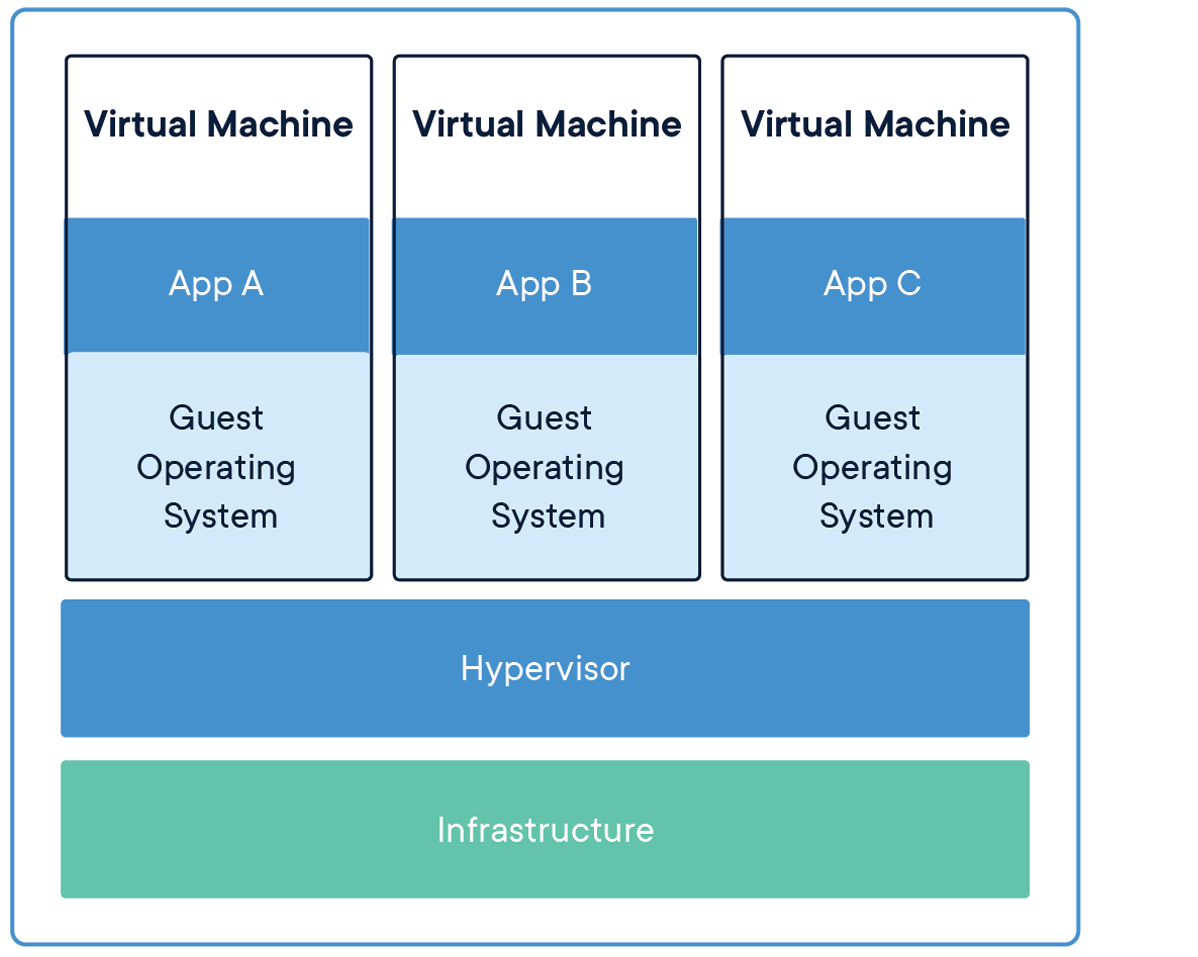
\includegraphics[width=0.5\linewidth]{vm_arch.png}
                    \caption[VM Setup]{Image portraying the general architecture of a VM-oriented setup. \cite{bib:vm-setup-img}.}
                    \label{fig:vm-arch}
                \end{figure}

            \subsubsection{Containers} \label{sec:container-intro}
                Before beginning to discuss whether containers are suitable for our purpose, we should begin by describing what a \textit{container} really is as it can be a confusing actor in the virtualization realm. Please note this section has been purposefully written as a high-level description of container technology. As stated before, a more technical discussion is presented on section \ref{sec:container-techy} belonging to chapter \ref{chap:2}.\\

                According to docker's documentation \cite{bib:docker-doc}, ``a \textit{container} is a standard unit of software that packages up code and all its dependencies so the application runs quickly and reliably from one computing environment to another''. Now, this definition is a perfect representative of the main kind of problems we will have to face when trying to bend containers to our will throughout the development process. Containers are designed to try and increase the portability of applications. In today's Internet-centric society, where we all want uninterrupted services, it is critical to be able to change an application's environment at a moment's notice due to outages, ending support cycles for software, security breaches... That is why the container technology has developed at such a high pace. It provides the infrastructure for a reliable service delivery. Now, we could ``twist'' the definition if we were to think of applications as full-fledged operating systems. That is, if we run a whole OS within these containers we would be actually achieving our goal: each container will behave as a network node so, in other words, we would only need to cope with $36$ concurrent containers: an easier task than doing the proper thing with VMs.\\

                One of the questions we asked ourselves when trying to decide on a technology was: what makes a container different than a VM? If we go back to the section we devoted to virtual machines we will notice how they run a full-fledged operating system as a guest. This implies each VM has its own \textit{kernel}. This is clearly shown on figure \ref{fig:vm-arch}.\\

                Kernels and their design have been the topic of many books and documents. We just need to know that the \textit{kernel} is the piece of software ``gluing'' the hardware and user-land software (programs such as browsers) together. That is, it allows applications to access the computing resources in an organized manner, enabling the sharing of resources amongst them. As we are telematics engineers we usually find the \textit{kernel} concept easier to understand in terms of the abstractions it offers us; the network socket being the most familiar. Through it, our applications can leverage the networking capabilities of the machine they're running on for instance.\\

                Unlike VMs, containers all share a single \textit{kernel}. We can then think of containers as a way of isolating applications along with all their dependencies within a shared computing platform. We don't need ``specialized'' software agents such as an hypervisor; we would only need to be very meticulous and know the \textit{kernel's} offered facilities very well to achieve the end result offered by containers. Projects like \textit{bocker} \cite{bib:bocker} prove one can achieve similar results to the ones provided by docker if only interested in a subset of the latter's capabilities. Nonetheless, one can regard containers as light VMs throughout the development as, even though it is not exactly true, it won't hinder our development approach. Figure \ref{fig:container-arch} shows the overall architecture of a container-based approach. Comparing it to figure \ref{fig:vm-arch} can be truly revealing when comparing both virtualization approaches.\\

                \begin{figure}
                    \centering
                    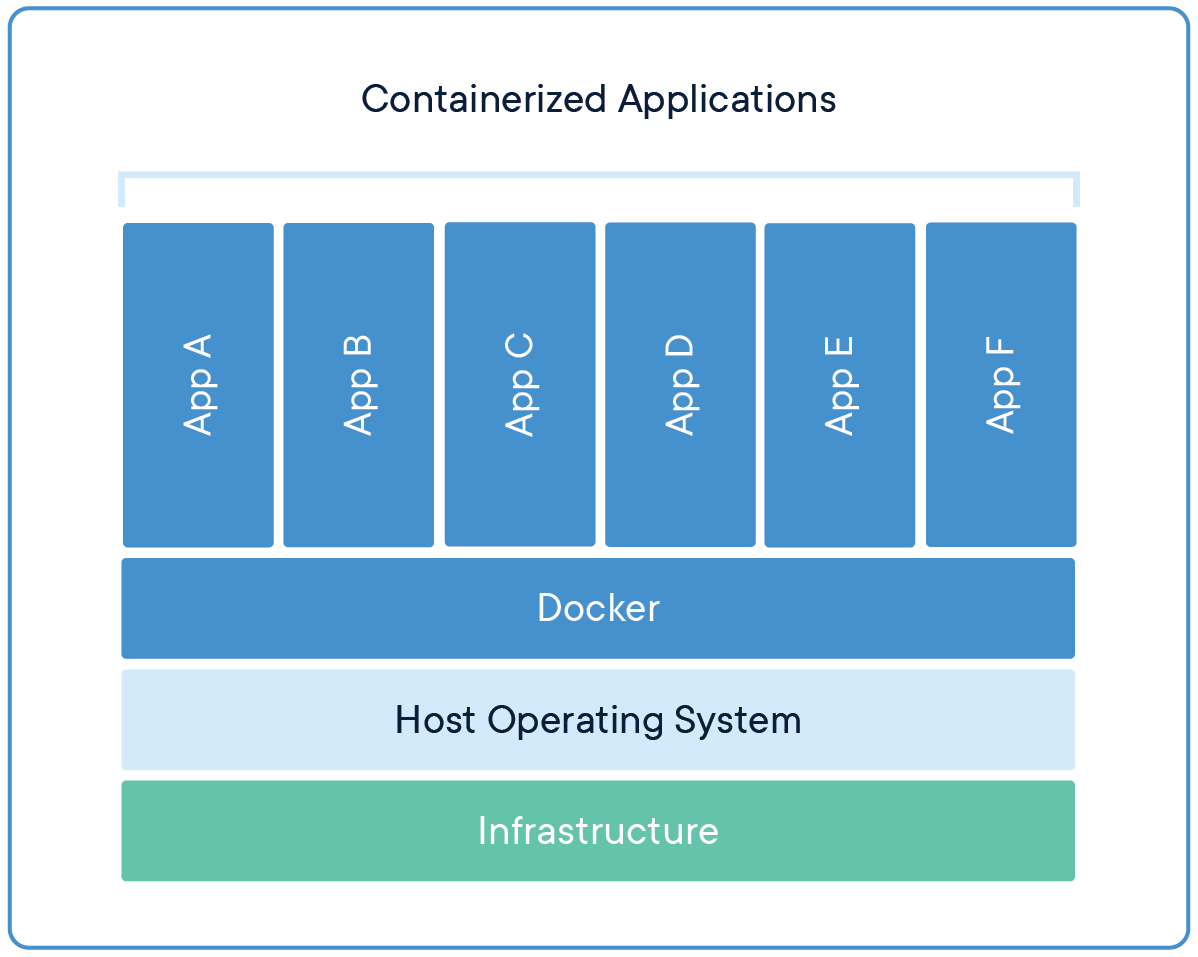
\includegraphics[width=0.5\linewidth]{container_arch.png}
                    \caption[Container Setup]{Image portraying the general architecture of a container-oriented setup. \cite{bib:container-setup-img}}
                    \label{fig:container-arch}
                \end{figure}

                \paragraph{Containers and Docker}
                    Container technology can be thought of as a standard. However, the way that technology is implemented can vary. Then, docker offers an \textit{implementation} for containers. This is a similar situation to that of VMs. The idea of a virtual machine has found two main implementations by VirtualBox and VMWare. This concept is similar to the situation posed by RFCs published by the IETF. They propose a standard and several people try to implement it according to their coding style, level of knowledge...

                    If we are to be entirely correct when it comes to nomenclature we would have to say that our solution is going to be based on docker's \textit{container implementation}.\\

                On top of container technology being lighter than that of VMs, which makes it more scalable, we also found the amount of documentation regarding the network infrastructure to be much larger. That gave us a strong foothold in our path to getting our framework up and running. Another positive aspect on containers we initially considered was the existence of \textit{container orchestration tools} such as \textit{Kubernetes} which we thought could make our job easier. We'll devote a few paragraphs to discussing why, in the end, \textit{Kubernetes} wasn't that much of a fit for us.

            \subsubsection{Kubernetes}
                As stated in \textit{Kubernetes'} own documentation \cite{bib:kubernetes-doc}, ``\textit{Kubernetes} is an open source container orchestration engine for automating deployment, scaling, and management of containerized applications''. In other words, \textit{Kubernetes} let's us define how we want our application to behave through a manifest provided in a \texttt{*.yaml} formatted file. Now, if we consider docker to be focused on offering ``services'', \textit{Kubernetes} takes that objective to the next level. It's a product aimed at professionals that's engineered to be stable. That means that meddling with the internals in an effort to achieve our goals was bound to be an extremely difficult task. By employing \textit{Kubernetes} we would be using an infrastructure that's already been laid for us, which is difficult to change and that does not behave how we want it to. We believe using a tool only to work against its basic principles is a wrong approach. That's why we decided to manually build the needed infrastructure from the ground up starting from docker containers.\\

                Just to give a concrete example of what we mean by working against the pre-existing infrastructure we could take a look at how \textit{Kubernetes} connects nodes. As it needs to offer some kind of service it will set up the internal network topology in such a way that all the nodes are able to connect among themselves. Given our requirement of implementing a firewall in the topologies we need to be working with, we can conclude it would be cumbersome to try to implement a firewall in an infrastructure whose primary concern is enabling communication links amongst all the network nodes. It's this diametrically opposite approach that made us dismiss \textit{Kubernetes} as a feasible solution.\\

        \subsection{Getting the Operating System}
            After settling on an option providing the ``hardware'' our software is to run on, we need to decide which operating system is the best suited for the task we have been proposed. Given today's ecosystem we quickly thought of the three main contenders in the user market. These are \textit{Microsoft Windows}, \textit{macOS} and \textit{Linux}. Before delving any deeper into the discussion about which to employ we would like to clarify our choice of words when referring to the last option.\\

            \paragraph{Linux vs. GNU/Linux}
                Strictly speaking, Linux is just the kernel of Linux-based distributions or \textit{distros}. As we explained in the previous section, a kernel is the piece of software gluing the hardware and user software together. It accomplishes this non-trivial feat by offering applications an interface through which they can request services. This kernel will then fulfill these requests in an orderly manner so that applications can coexist and cooperate towards a better overall usage of the system. These applications can in fact not even be aware that they are running alongside others.

                The kernel is for many the most crucial piece of software within a full fledged operating system. It's the cornerstone on which everything else is built. Nonetheless, if a non-technical user were given just a kernel they would have a very hard time making any use of it. This is where applications or user programs come into play. The make use of the OS's services and they let an end-user get meaningful work done. These end user programs range form text editors such as \texttt{vim} or \texttt{Microsoft Word} to VoIP (Voice over IP) PBXs (Private Branch eXchanges) like \texttt{asterisk}.

                The role of GNU in all this is providing many of these end user programs as free (as in freedom) software. Huge projects like the \texttt{gnome} desktop environment and \texttt{make} (which we are using for compiling this \LaTeX file) carry the GNU stamp. Given the above, GNU argues operating systems packaging their tools should be considered GNU/Linux systems as these two terms work cooperatively, i.e. they are software pieces with distinct purposes. While we consider this to be absolutely true for end-user systems such as \texttt{Ubuntu desktop} and \texttt{Debian} we feel this is not the real case with us.

                We will be running our network nodes as docker containers and we will try to make the image ran by these containers as lightweight as possible. In doing that we will only rely on GNU's shell, \texttt{bash}, for running a very restricted collection of commands. That is why we will refer to our platform as Linux containers instead of GNU/Linux ones.

            Knowing we have already restricted ourselves to the use of container technology we can discard \textit{macOS} as an option right away as there is no official support for it. We could have used \textit{Windows}-based containers but given our uncommon requirements we opted to use a \textit{linux}-based one. Given we feel comfortable with it, we settled on using \textit{Ubuntu} docker images for running our nodes. The version we employed during the testing phase was deemed \texttt{Bionic Beaver} and had version number \texttt{18.04 LTS} (Long Term Release) which boasts a higher stability than yearly versions. Given our requirements, all our work should run ``just fine'' on newer versions. We nonetheless recommend working to \texttt{LTS} releases as the yearly builds can sometimes behave unexpectedly. On top of our choice's flexibility, we mustn't forget about the price and licensing factors. Even though we haven't looked into these topics regarding Microsoft's OS, Windows licenses tend to be more restrictive than those attached to Ubuntu. As we plan on working at a very ``low level'' with the kernel's internal network infrastructure we aren't entirely sure if that would be allowed by Window's license terms. On top of that Ubuntu doesn't cost anything, so we won't have to be concerned about a monetary budget. Putting it all together justifies why we decided to run Ubuntu within our own containers.
